\documentclass[a4paper]{article}
\usepackage[pdftex]{hyperref}
\usepackage[latin1]{inputenc}
\usepackage[english]{babel}
\usepackage{a4wide}
\usepackage{amsmath}
\usepackage{amssymb}
\usepackage{algorithmic}
\usepackage{algorithm}
\usepackage{ifthen}
\usepackage{listings}
\usepackage{array}
\usepackage{tabu}
% move the asterisk at the right position
\lstset{basicstyle=\ttfamily,tabsize=4,literate={*}{${}^*{}$}1}
%\lstset{language=C,basicstyle=\ttfamily}
\usepackage{moreverb}
\usepackage{palatino}
\usepackage{multicol}
\usepackage{tabularx}
\usepackage{comment}
\usepackage{verbatim}
\usepackage{color}
\usepackage{graphicx}
\usepackage{array,mathtools}
\usepackage{amsmath}
\usepackage{enumitem,amssymb}
\usepackage{pifont}
\newlist{todolist}{itemize}{2}
\setlist[todolist]{label=$\square$}
\newcommand{\cmark}{\ding{51}}%
\newcommand{\xmark}{\ding{55}}%
\newcommand{\done}{\rlap{$\square$}{\raisebox{2pt}{\large\hspace{1pt}\cmark}}%
\hspace{-2.5pt}}
\newcommand{\wontfix}{\rlap{$\square$}{\large\hspace{1pt}\xmark}}



%% pdflatex?
\newif\ifpdf
\ifx\pdfoutput\undefined
\pdffalse % we are not running PDFLaTeX
\else
\pdfoutput=1 % we are running PDFLaTeX
\pdftrue
\fi
\ifpdf
\fi
\ifpdf
\DeclareGraphicsExtensions{.pdf, .jpg}
\else
\DeclareGraphicsExtensions{.eps, .jpg}
\fi

\parindent=0cm
\parskip=0cm

\setlength{\columnseprule}{0.4pt}
\addtolength{\columnsep}{2pt}

\addtolength{\textheight}{5.5cm}
\addtolength{\topmargin}{-26mm}
\pagestyle{empty}

%%
%% Sheet setup
%% 
\newcommand{\coursename}{Computer Architecture and Programming Languages}
\newcommand{\courseno}{CO20-320241}
\newcommand*{\carry}[1][1]{\overset{#1}}
\newcolumntype{B}[1]{r*{#1}{@{\,}r}}
 
\newcommand{\sheettitle}{Homework}
\newcommand{\mytitle}{}
\newcommand{\mytoday}{{18th of November}, 2019}

% Current Assignment number
\newcounter{assignmentno}
\setcounter{assignmentno}{9}

% Current Problem number, should always start at 1
\newcounter{problemno}
\setcounter{problemno}{1}

%%
%% problem and bonus environment
%%
\newcounter{probcalc}
\newcommand{\problem}[2]{
  \pagebreak[2]
  \setcounter{probcalc}{#2}
  ~\\
  {\large \textbf{Problem \textcolor{blue}{\arabic{assignmentno}}.\textcolor{blue}{\arabic{problemno}}} \hspace{0.2cm}\textit{#1}} \refstepcounter{problemno}\vspace{2pt}\\}

\newcommand{\bonus}[2]{
  \pagebreak[2]
  \setcounter{probcalc}{#2}
  ~\\
  {\large \textbf{Bonus Problem \textcolor{blue}{\arabic{assignmentno}}.\textcolor{blue}{\arabic{problemno}}} \hspace{0.2cm}\textit{#1}} \refstepcounter{problemno}\vspace{2pt}\\}

%% some counters  
\newcommand{\assignment}{\arabic{assignmentno}}

%% solution  
\newcommand{\solution}{\pagebreak[2]{\bf Solution:}\\}

%% Hyperref Setup
\hypersetup{pdftitle={Homework \assignment},
  pdfsubject={\coursename},
  pdfauthor={},
  pdfcreator={},
  pdfkeywords={Computer Architecture and Programming Languages},
  %  pdfpagemode={FullScreen},
  %colorlinks=true,
  %bookmarks=true,
  %hyperindex=true,
  bookmarksopen=false,
  bookmarksnumbered=true,
  breaklinks=true,
  %urlcolor=darkblue
  urlbordercolor={0 0 0.7}
}

\begin{document}


\coursename \hfill Course: \courseno\\
Jacobs University Bremen \hfill \mytoday\\
Fjolla Dedaj\hfill
\vspace*{0.3cm}\\
\begin{center}
{\Large \sheettitle{} \textcolor{blue}{\assignment}\\}
\end{center}
\problem{}{0}
\textbf{(a) Why does the PC not need an explicit write signal in a single-cycle datapath?}\\
\solution
If you check the single cycle control signals flowing in this question, the Jump and Branch control signals feed the muxes at the end of the pipeline, which determines the input to the PC. In the absence of these control inputs, the PC will be incremented by its default value, 4. Therefore there is no need of an explicit write control for PC in a single cycle data path.\\
\\
\textbf{(b) Why is an explicit write control signal needed in a multicycle datapath?}\\
\solution
This happens because there are a lot of operations happening in parallel, therefore, explicit control is necessary to determine which path to pick in determining the address of the next instruction.\\


\problem{}{0}
\\
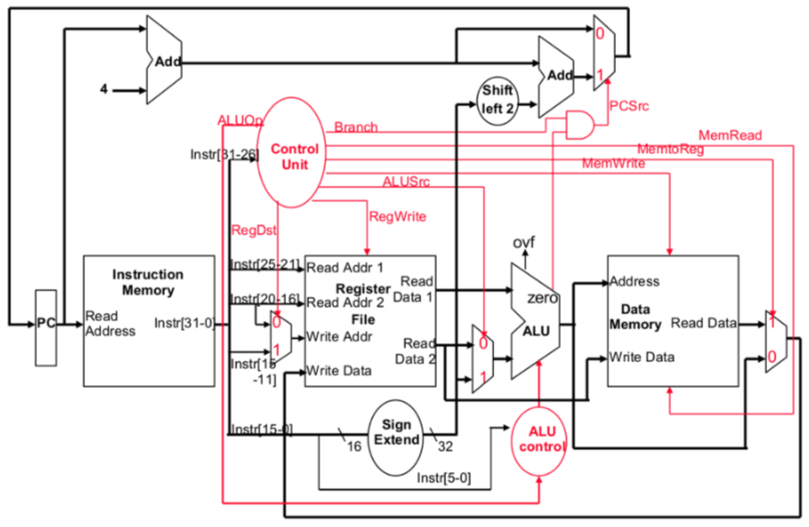
\includegraphics[scale=0.45]{2.png}\\
\\
(a) By marking (by e.g., a thicker line or another color) the active lines and circling the active selectors in the figure above, show the single-cycle datapath for the add \$s0 \$s1 \$s2 and lw \$s3 16 (\$s2)instructions. Use two copies of the figure for the two instructions. Then with your findings write down the values of the control lines for the instructions into the table below.\\
\\
\pagebreak
\\
\solution
\\
\textbf{add \$s0 \$s1 \$s2:}\\
\\
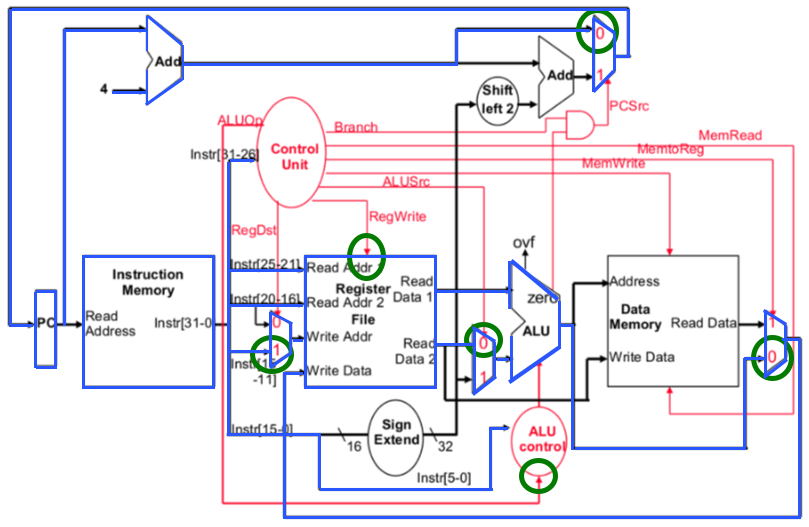
\includegraphics[scale=0.45]{2a1.png}
\\
\textbf{lw \$s3 16 (\$s2):}\\
\\
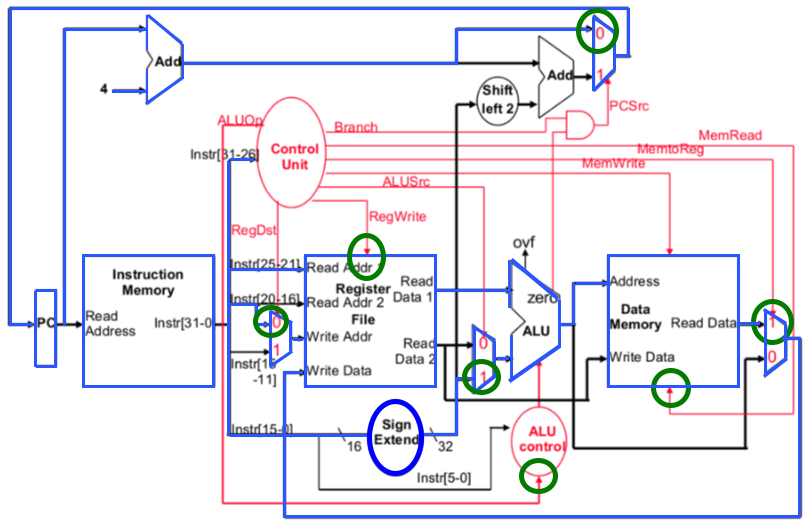
\includegraphics[scale=0.45]{2a2.png}\\
\\
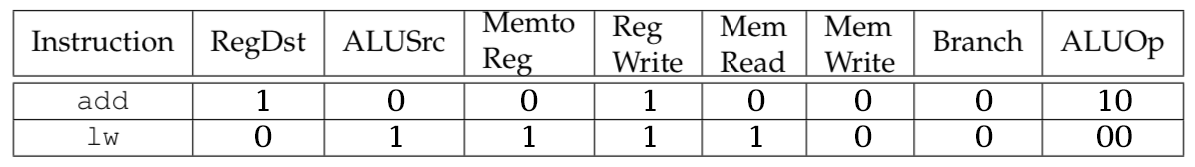
\includegraphics[scale=0.35]{2b.png}\\
\\
(b) When does the ALU need to add its inputs? Give and explain detailed examples from at least two different instruction classes.\\
\\
The ALU will perform add operation when the ALU control input is exactly 0010. This happens when lw or sw are executed and the ALUOp is 00.
Or add/sub are executed and the ALUOp os 10.
When these operations happen, the operands in the ALU go through addition, but for different usages. For add it will only do the sum of two values, while for lw and sw you need to add the base address of a register and the offset.

\end{document}